\section{Zweidimensionales Punktediagramm}

Da das zweidimensionale Punktediagramm weit verbreitet ist, sind sich Betrachter an diese Darstellung gewöhnt. Oft werden die Punkte in Diagramm durch eine Linie verbunden, was den Verlauf der abgebildeten Datenwerte verdeutlicht, besonders in Medien, zum Bespiel für die Darstellung von Börsenkursen. 

Aus diesem Grund wurde als erstes Beispiel das zweidimensionale Punktediagramm (beziehungsweise das Liniendiagramm, falls Linien hinzugefügt werden) ausgewählt.

\subsection{Information-Seeking Mantra}

Als Startreferenz für die Entwicklung des interaktiven Diagrammes bieten sich die von Ben Shneiderman begründeten Prinzipien für das Design graphischer Benutzeroberflächen an, das "`\textit{Information-Seeking Mantra}"'. Die Weise, wie der Benutzer mit der Oberfläche interagiert, hat Shneiderman \cite{shneiderman} festgelegt:

\begin{itemize}
	\item Überblick ("`\textit{Overview first}"')
	\item Zoomen und Filtern ("`\textit{zoom and filter}"')
	\item Details auf Abruf ("`\textit{then details-on-demand}"')
\end{itemize}

\textbf{Überblick.} Der Benutzer verschafft sich einen Überblick über die gesamte Oberfläche des Programms.

\textbf{Zoom.} Zur besseren Betrachtung vergrössert der Benutzer die Ansicht, sodass die betreffenden Elemente grösser angezeigt werden.

\textbf{Filter.} Die Filter-Funktion ermöglicht dem Benutzer, gewisse Elemente oder Elementgruppen je nach Interesse ein- oder auszublenden.

\textbf{Details auf Abruf.} Falls ein Element den Nutzer besonders interessiert, besteht die Möglichkeit, dass zusätzliche relevante Informationen zum Element angezeigt werden können.

Zusätzlich formulierte Shneiderman drei weitere Schritte:

\textbf{Zusammenhänge betrachten.} Die Zusammenhänge zwischen den verschiedenen Elementen können im Programm betrachtet werden. Diesen Schritt umzusetzen ist nur bei wenigen Benutzeroberflächen sinnvoll, zum Beispiel bei der Darstellung von Baumdiagrammen oder anderen Diagramme mit hierarchischen Daten.

\textbf{Verlauf.} Die Interaktionen des Benutzers mit der Programmoberfläche werden aufgezeichnet. Dadurch können Interaktionen rückgängig gemacht werden.

\textbf{Extraktion.} Damit wird die Extraktion erlaubt der \textit{Query-Parameter} (wie angewandte Filter, Verlauf, Zoomstufe) und der durch die Interaktion bereits definierten Elementgruppen ("`\textit{subcollections}"').

Im Diagramm werden nur die Methoden \textit{Überblick}, \textit{Zoom}, \textit{Filter} und \textit{Details auf Abruf} umgesetzt. Das Mantra wurde allgemein für Benutzeroberflächen von Programmen beschrieben, in unserer Applikation, einem interaktiven Diagramm, macht aber die Umsetzung der Schritte \textit{Zusammenhänge betrachten}, \textit{Verlauf}, \textit{Extraktion} in Bezug auf die Funktion des Diagramms keinen Sinn:

\begin{itemize}
	\item Punktediagramme oder Liniendiagramme werden nicht dazu verwendet, Daten in Hierarchieform darzustellen.
	\item Die Interaktionen im Diagramm sind zu banal, als dass eine Rückgängig-Funktion von Nutzen wäre.
	\item Die Extraktion und der Export von Query-Parametern des Diagramms ist zwar theoretisch umzusetzen, ist jedoch von minimaler praktischer Bedeutung.
	\item Zur Extraktion von "`\textit{subcollections}"' aus einem Datensatz sollte kein interaktives Diagramm verwendet werden. Eine Datenverarbeitungsapplikation ist für diese Aufgabe angemessener, da exakte Parameter zur Extraktion bestimmt werden können.
\end{itemize}

\newpage

\subsection{Applikation}

\begin{figure}[!htbp]
	\centering
	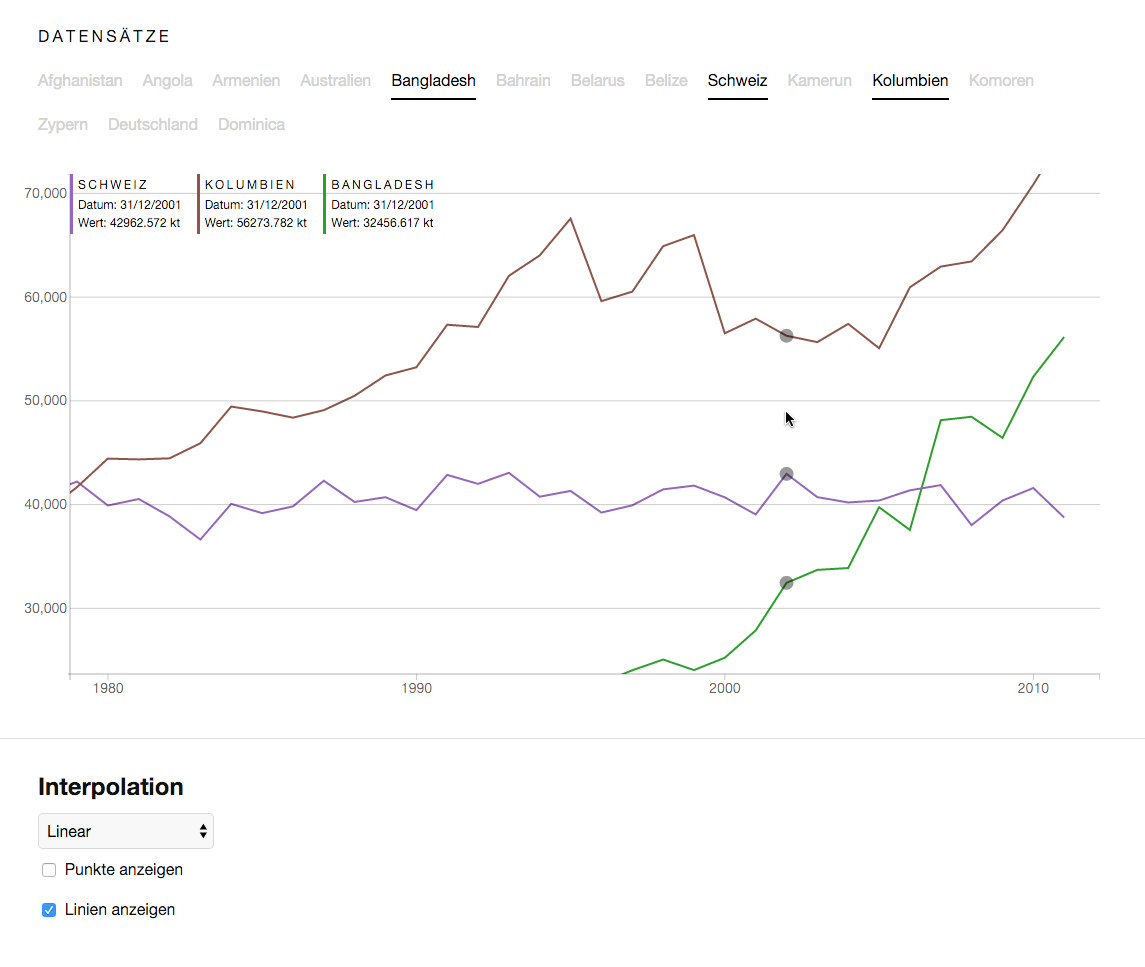
\includegraphics[width=\linewidth]{images/2dline}
	\caption{Screenshot der Oberfläche der Applikation (zweidimensionales Liniendiagramm / Punktediagramm)}
	\label{fig:screenshot}
\end{figure}

Der Screenshot in Abbildung \ref{fig:screenshot} zeigt die entwickelte Applikation. Es sind Datensätze \cite{worldbank} zum $CO_2$-Verbrauch von 15 Ländern vorhanden, drei davon sind im Diagramm eingeblendet.

\textbf{Achsen.} Es wurden Achsen mit linearer Skala für die Applikation gewählt. Beschriftungen, sogenannte \textit{Ticks}, sind vorhanden. Die Ticks auf der Ordinatenachse (y-Achse) wurden in Richtung der Innenseite des Diagramms verlängert, so dass ein Gitter entsteht.

Falls in einem Diagramm mehrere Datensätze gleichzeitig dargestellt werden sollen, wie es der Fall in Abbildung \ref{fig:screenshot} ist, so müssen die abgebildeten Werte die gleiche Einheit (zum Beispiel Meter, Kilogramm, Franken) besitzen. Bei der gleichzeitigen Darstellung von mehreren Datensätzen mit verschiedenen Einheiten in einem Diagramm muss für jede vorhandene Einheit eine eigene Achse und Skala gezeichnet werden.

\textbf{Datenpunkte.} Die Applikation bietet an, die Daten als Punkte und bzw. oder verbunden durch eine Linie anzuzeigen. In Abbildung \ref{fig:screenshot} unten wird durch Kontrollkästchen ermöglicht, die Anzeige zu verändern.

\textbf{Layout und Textformatierung.} Für den Schritt \textit{Übersicht} ist das Layout und auch die Formatierung des Textes von Bedeutung. Eine klare Oberflächenstruktur nach modernen Minimalismus (nach Designtrends wie \textit{Flat Design} oder \textit{Material Design}) wurde geschaffen, bei denen der Inhalt im Vordergrund steht. "`Benutzer betrachten keine Details, sie benutzen Details."' \cite{minimalism}.

Zur besseren Orientierung des Benutzers wird hier das Prinzip von "`\textit{pop}"' und "`\textit{unpop}"' von Text, das von Erik Kennedy \cite{pop} beschrieben wurde, berücksichtigt: Durch die Anpassung der Typographie kann ein Text hervorgehoben, beziehungsweise in den Hintergrund gestellt werden. Folgende Eigenschaften von Texten im Diagramm werden in der Applikation entsprechend der Wichtigkeit angepasst:

\begin{itemize}
	\item Grösse (grösser bzw. kleiner)
	\item Farbe (grösser bzw. kleinerer Kontrast)
	\item Schriftstärke (fetter bzw. leichter)
	\item Schriftart (Grossschreibung bzw. Kleinschreibung)
	\item Laufweite (kleiner bzw. grösser)
	\item Unterstreichung (unterstrichen bzw. nicht unterstrichen)
\end{itemize}

\textbf{Linien.} Der Verlauf der abgebildeten Datenwerte wird verdeutlicht, indem die Punkte im Diagramm durch eine Linie verbunden werden. Die lineare Interpolation wurde durch ein selbstgeschriebenes Modul implementiert. Weitere Interpolationen, wie der \textit{Kubisch Hermitescher Spline} oder \textit{Basis-Spline}, wurden mit D3 implementiert und können auf das Diagramm angewendet werden.

\begin{figure}[!htbp]
	\begin{minipage}{\textwidth}
		\centering
		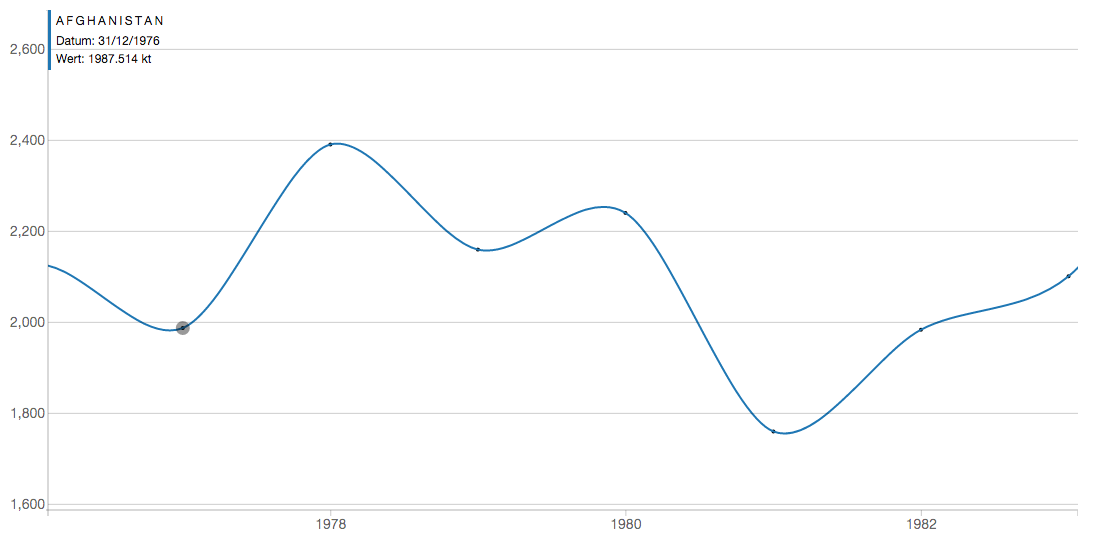
\includegraphics[width=\linewidth]{images/cardinal}
	\end{minipage}
	\begin{minipage}{\textwidth}
		\centering
		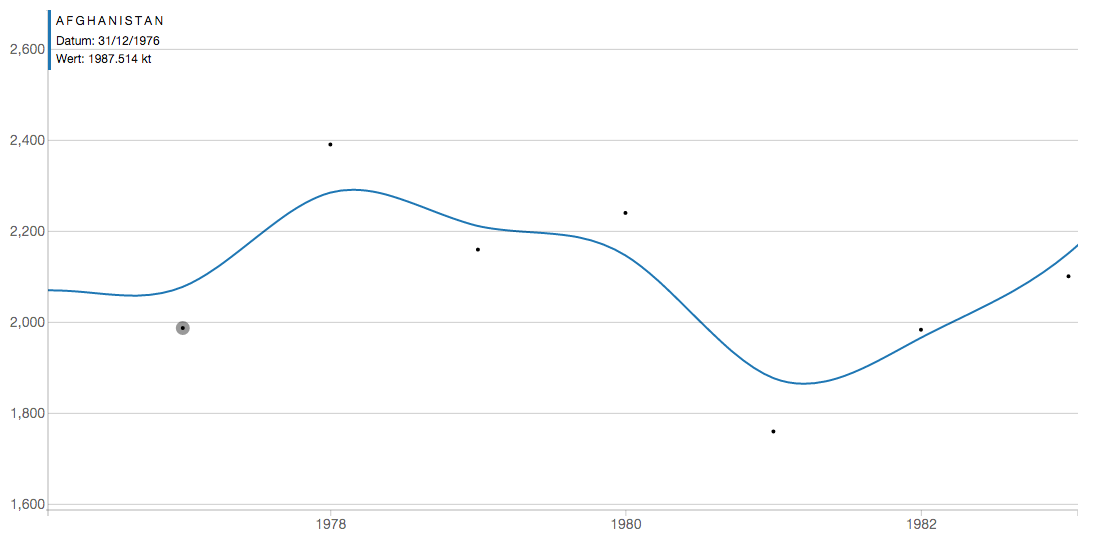
\includegraphics[width=\linewidth]{images/basis}
	\end{minipage}
	\caption[Beispiele von Interpolationen und Zoom]{1. Beispiele von Interpolationen im Diagramm. V.o.n.u: Kubisch Hermitescher Spline, Basis-Spline. 2. Gezoomte Ansicht}
	\label{fig:vergleich}
\end{figure}

Verschiedene Farben von Linien ermöglichen die Zuordnung von Datensätzen. Die den Datensätzen zugewiesenen Farben werden in der Detailanzeige dargestellt.

\textbf{Zoom.} Der Schritt \textit{Zoomen} wurde im Diagramm umgesetzt. Es kann durch Scrollen gezoomt werden. Die Programmlogik wurde mittels D3 implementiert.

\textbf{Datensatzauswahl.} In diesem Beispiel (Abbildung \ref{fig:screenshot}) können Linien ein- und ausgeblendet werden, die Datensätzen für 15 Länder entsprechen. Dieser Vorgang gehört zum Schritt \textit{Filtern}. Aktivierte, angezeigte Datensätze werden nach den Prinzipien von Kennedy hervorgehoben, nicht aktivierte, versteckte Datensätze sind in den Hintergrund gestellt.

\textbf{Tooltip und Detailanzeige.} Beim Tooltip wird der der Maus am nächsten liegende Datenpunkt jedes Datensatzes markiert und erscheint in der Detailanzeige. In der Detailanzeige werden, falls im Datensatz vorhanden, weitere Informationen (Datenspalten) und genaue x- und y-Werte mit Einheit angezeigt. Dieser Vorgang entspricht dem Schritt \textit{Details auf Abruf}.

\textbf{Dynamik der Applikation.} Der Screenshot dieses Beispiels (Abbildung \ref{fig:screenshot}) ist das Resultat der Anzeige der Applikation, die für einen bestimmten Datensatz konfiguriert ist. Elemente des Diagramms, wie der Wertebereich der Achsen, die Datensatzauswahl, Tooltip, Detailanzeige, werden dynamisch generiert, so dass diese Module ohne weitere Einstellung auch für andere Datensätze funktionieren.

